\section{Mineração de Dados}
\label{sec:data-mining}

A mineração de dados é abordada na literatura como a principal etapa do processo de KDD, nela ocorre a busca por conhecimento útil nas bases de dados, levando autores a referenciar ambos como sendo sinônimos. Segundo \citeonline{passos2005data}, a fase de mineração, em sua execução, compreende a aplicação de algoritmos sobre os dados, buscando abstrair o conhecimento presente. Tais algoritmos são fundamentados em técnicas que têm como objetivo explorar os dados, produzindo modelos de conhecimento a partir deles. A maneira como o conhecimento destes modelos é representado depende do algoritmo de mineração aplicado.

De acordo com \citeonline{fayyad1996kdd}, algoritmos de mineração de dados são compostos de três componentes básicos, são eles: a tarefa; o critério da tarefa; e o algoritmo de busca. As tarefas de mineração são escolhidas de acordo com o propósito da aplicação e são observados dois fatores relevantes: a tarefa em si e a representação da mesma, que refere\hyp{}se a representação dos dados e sua interpretabilidade.

\begin{figure}[H]
    \centering
    \caption{Base de dados Iris utilizada em tarefas de \textit{clustering}.}
    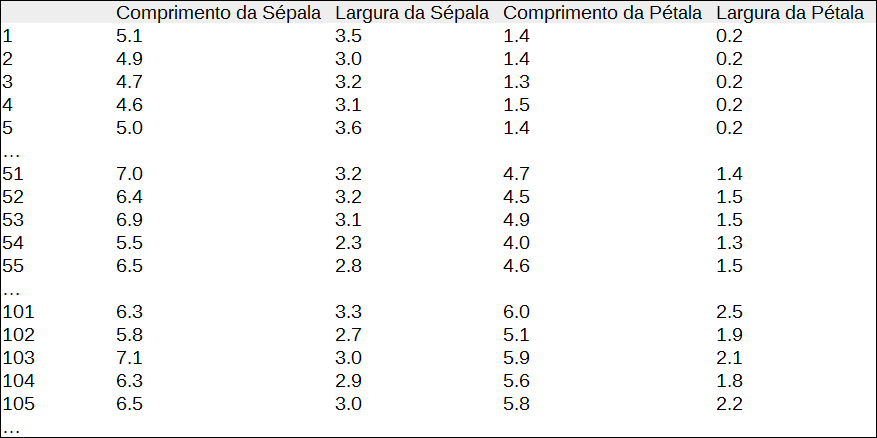
\includegraphics[width=0.9\linewidth]{figuras/iris-clustering.png}
    \source{Adaptado de \cite{witten2011data}.}
    \label{fig:iris-clustering}
\end{figure}

As tarefas de mineração são amplamente definidas por diversos autores. A seguir, pode\hyp{}se observar as mais comuns, juntamente com exemplos de suas aplicações:

\begin{enumerate}[label=\roman*.]
    \item Análise de agrupamentos {--} Para um número de exemplos em uma base de dados, caracterizados por conjuntos de atributos, como pode ser observado no exemplo representado pela Figura \ref{fig:iris-clustering}, esta técnica busca separar os indivíduos dividindo\hyp{}os em agrupamentos (\textit{clusters)}. As instâncias que formam um agrupamento são similares entre si e se distinguem de outras instâncias em agrupamentos diferentes. A separação destas instâncias ocorre a partir do cálculo de similaridade entre os atributos dos dados. Utiliza\hyp{}se análise de agrupamento quando não existem classes pré\hyp{}definidas e os dados devem ser divididos em grupos (\textit{e.g.} compreender as ações de indivíduos em um ambiente escolar);
    \item Classificação {--} Dado um número de exemplos, como apresentados na Figura \ref{fig:iris-classification}, esta técnica busca atribuir rótulos pré\hyp{}estabelecidos para instâncias em que esta informação não é conhecida. A rotulagem ocorre baseada na análise das características dos exemplos onde a classe é conhecida. Classificação é usada para determinar a que modelo pré\hyp{}existente pertence uma nova instância (\textit{e.g.} para a base Iris, identificar o sub-tipo de uma flor);
    
    \begin{figure}[H]
        \centering
        \caption{Base de dados Iris utilizada em tarefas de classificação.}
        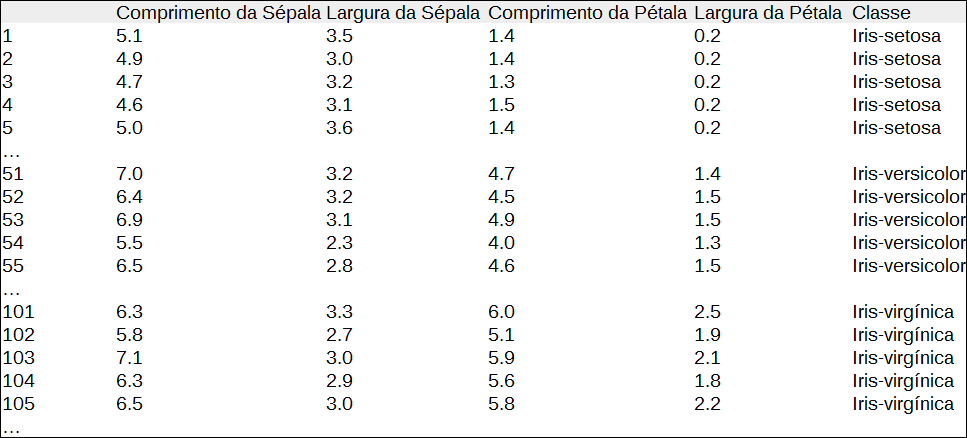
\includegraphics[width=0.9\linewidth]{figuras/iris-classification.png}
        \source{Adaptado de \cite{witten2011data}.}
        \label{fig:iris-classification}
    \end{figure}
    
    \item Detecção de anomalias {--} Observa instâncias que apresentam disparidade do conjunto de dados em que estão inseridas, identificando anomalias através do cálculo de similaridade entre os elementos da base. O estudo dos dados que se distinguem do restante da base, também conhecidos como \textit{outliers}, pode fornecer informações mais interessantes do que o estudo de uma grande quantidade de dados uniforme. Utiliza\hyp{}se detecção de anomalias quando se deseja reconhecer elementos cujas ações estão fora de um padrão esperado (\textit{e.g.} investigação de fraudes em cartões de crédito);
    \item Regras de associação {--} Esta tarefa busca representar associações entre instâncias num banco de dados. As associações são utilizadas para prever a aparição de um item dependendo da existência de outros. As regras criadas devem atingir um valor mínimo de suporte e confiança, onde o primeiro (suporte) remete a quantidade de aparições da regra na base, enquanto o segundo (confiança) se refere a quantidade de vezes que o caso foi observado como verdadeiro. Regras de associação são utilizada quando se deseja verificar a dependência entre itens, identificando padrões que poderiam permanecer ocultos para outras tarefas de mineração (\textit{e.g.} utilizada no comércio, onde busca identificar itens comprados em conjunto).
\end{enumerate}